\chapter{Planning}

\subsection{Planning fase overview}
The first fase of this project involved a lot of planning. It was necessary to get an overview over the hours avilable and how much all the team members was prepared to work. In addition to this all the milestones in this project and the amount of total time the team wanted to use on each of the different aspects of the project was discussed.


\newpage
\input ch/planning/sec/wbs.tex

\newpage
\subsection{Gantt diagram}

A Gantt diagram is a representation of all the work hours, milestones and deadlines that is involved in a project. The Gantt diagram for our project is given in figure~\ref{fig:gantt}.

\begin{figure}[H]
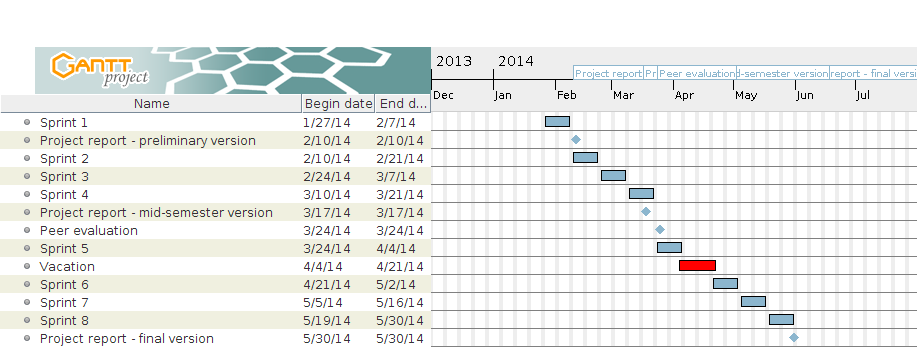
\includegraphics[width=\textwidth]{ch/planning/fig/gantt.png}
\caption{The Gantt diagram with sprints and milestones.}
\label{fig:gantt}
\end{figure}

\input ch/planning/sec/agileDevelopment.tex
\input ch/planning/sec/scrum.tex
\input ch/planning/sec/extremeProgramming.tex

\input ch/planning/sec/risk.tex
%\input ch/planning/sec/architecture.tex
